\documentclass[12pt]{article}
\usepackage{amsmath}
\usepackage{amssymb}
%\usepackage{hyperref}
\usepackage{epsfig,graphicx,amsmath}
\usepackage{amsfonts}
\usepackage{enumerate}
\usepackage{amsfonts}
\usepackage{amssymb}
\usepackage{amsthm}


\newcommand{\mb}[1]{\mbox{\boldmath$#1$}}
\newcommand{\p}{\partial}
\newcommand{\ds}{\displaystyle}
\newcommand{\beq}{\begin{eqnarray}}
\newcommand{\beqq}{\begin{eqnarray*}}
\newcommand{\eeq}{\end{eqnarray}}
\newcommand{\eeqq}{\end{eqnarray*}}
\newcommand{\eps}{\varepsilon}
\newcommand{\erf}{\mbox{erf}}
\newcommand{\erfi}{\mbox{erfi}}
\newcommand{\Ei}{\mbox{Ei}}
\newcommand{\x}{\mbox{\boldmath$x$}}
\newcommand{\Aa}{\mbox{\boldmath$A$}}
\newcommand{\rr}{\mbox{\boldmath$r$}}
\newcommand{\As}{\mbox{\boldmath$a$}}
\newcommand{\y}{\mbox{\boldmath$y$}}
\newcommand{\z}{\mbox{\boldmath$z$}}
\newcommand{\J}{\mbox{\boldmath$J$}}
\newcommand{\ET}{\mbox{\boldmath$\eta$}}
\newcommand{\n}{\mbox{\boldmath$n$}}
\newcommand{\X}{\mbox{\boldmath$X$}}
\newcommand{\Y}{\mbox{\boldmath$Y$}}
\newcommand{\Yy}{\mbox{\boldmath$y$}}
\newcommand{\Z}{\mbox{\boldmath$Z$}}
\newcommand{\w}{\mbox{\boldmath$w$}}
\newcommand{\vv}{\mbox{\boldmath$v$}}
\newcommand{\bb}{\mbox{\boldmath$b$}}
\newcommand{\Bb}{\mbox{\boldmath$b$}}
\newcommand{\B}{\mbox{\boldmath$B$}}
\newcommand{\ALPHA}{\mbox{\boldmath$\alpha$}}
\newcommand{\aaa}{\mbox{\boldmath$a$}}
\newcommand{\C}{\mbox{\boldmath$C$}}
\newcommand{\SSigma}{\mbox{\boldmath$\Sigma$}}
\newcommand{\mmu}{\mbox{\boldmath$\mu$}}
\newcommand{\IIm}{\mbox{\boldmath$I_m$}}
\newcommand{\mean}[1]{\langle #1\rangle}
\newcommand{\diffunit}{$\mu$m$^2$.s$^{-1}$}
\newcommand{\Li}{\mbox{Li}}
\newcommand{\thet}{\mbox{\boldmath$\theta$}}
\newcommand{\intR}{\int\limits_{\mathbb{R}}}
\newcommand{\intRm}{\int\limits_{\mathbb{R}^m}}
\newcommand\norm[1]{\left\lVert#1\right\rVert}
%\definecolor{red}{rgb}{1,0,0}

\usepackage{color}
\usepackage{float}
\begin{document}	
\title{Results \& Material and methods}
\author{Ofir Shukron \& David Holcman}
\maketitle

\section{Result section}

To estimate the nucleosome reorganization following DNA damages, we have constructed a model where redistribution can be due either to chromatin de-compaction or nucleosome sliding along the chromatin or both of them. We have used the model to assess the relative contribution of these two processes to the total signal loss from a region of interest (ROI), a quantity which is inaccessible experimentally. 

The model (presented in Material and methods) follows the DNA, $D(u)$, and nucleosome, $H(u)$, fraction of signal loss from the ROI as a function of the UV dose, $u$. We have used the measured H3.3 and DNA signal loss to calibrate parameters of nucleosome and DNA models respectively (Fig. 3A-D). Using the calibrated models we find that the relative contribution of nucleosome sliding to the total signal loss in the ROI is monotonically decreasing from 70\% to 64 \% for nucleosomes and 43 to 41\% for DNA loss, as the UV dose increases from 5 to 100 msec. The remaining percentages are attributed to chromatin expansion and de-compaction (see figure \ref{fig:relatiiveContributionToLoss}).

\begin{figure}[H]
	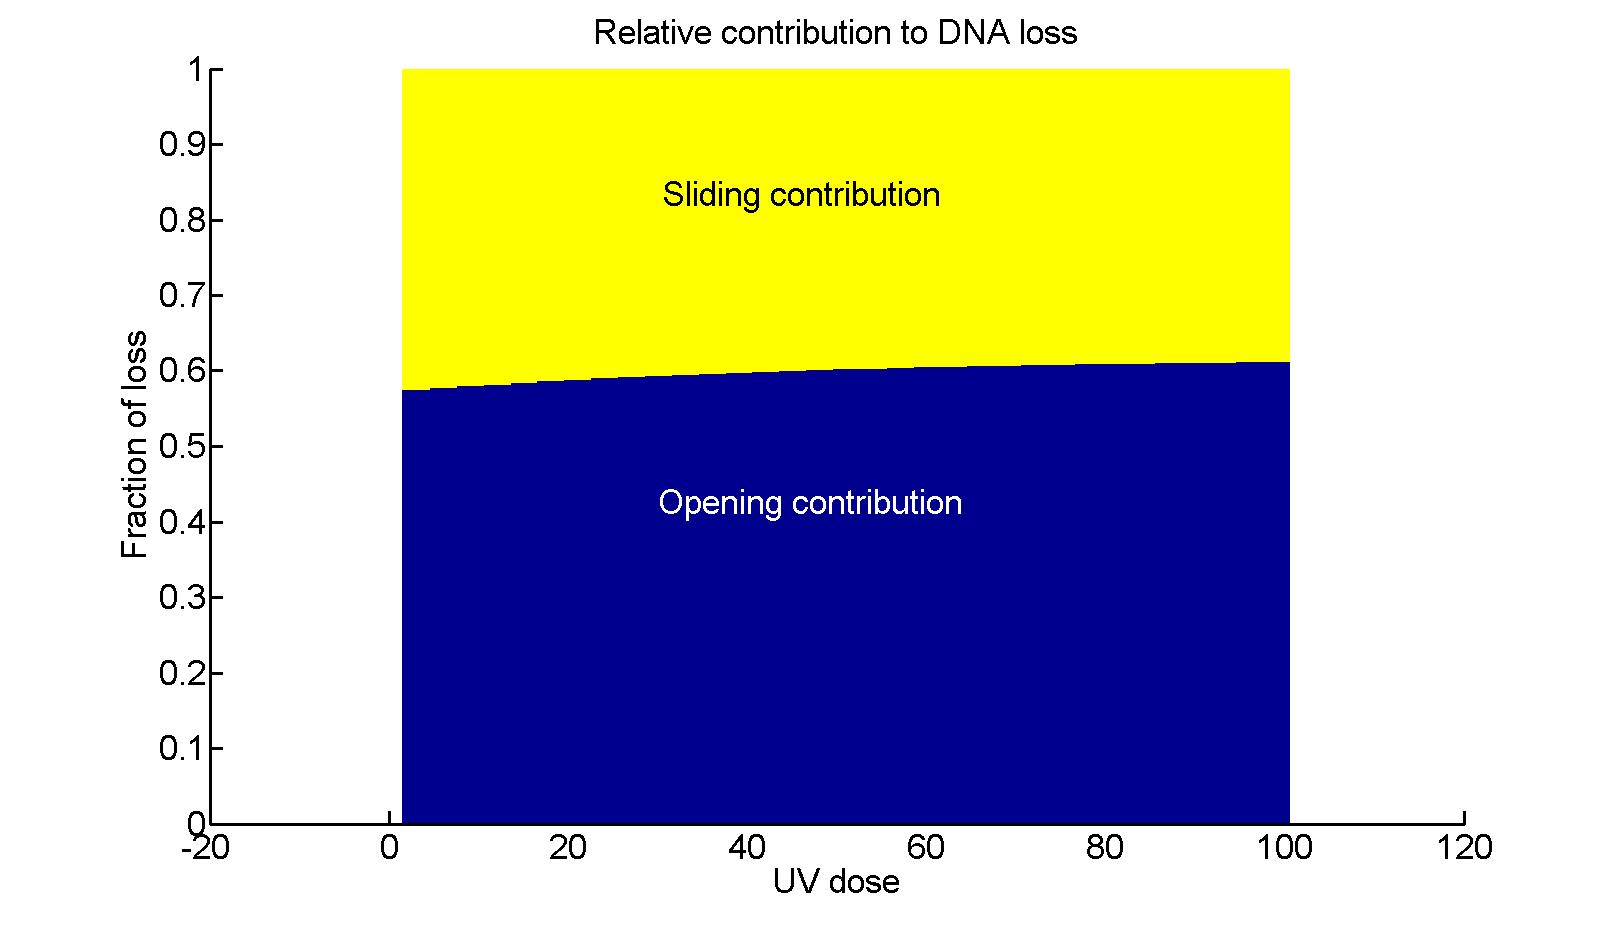
\includegraphics[width=0.5\linewidth, height=0.3\textheight]{relatiiveContributionToDNALoss}
	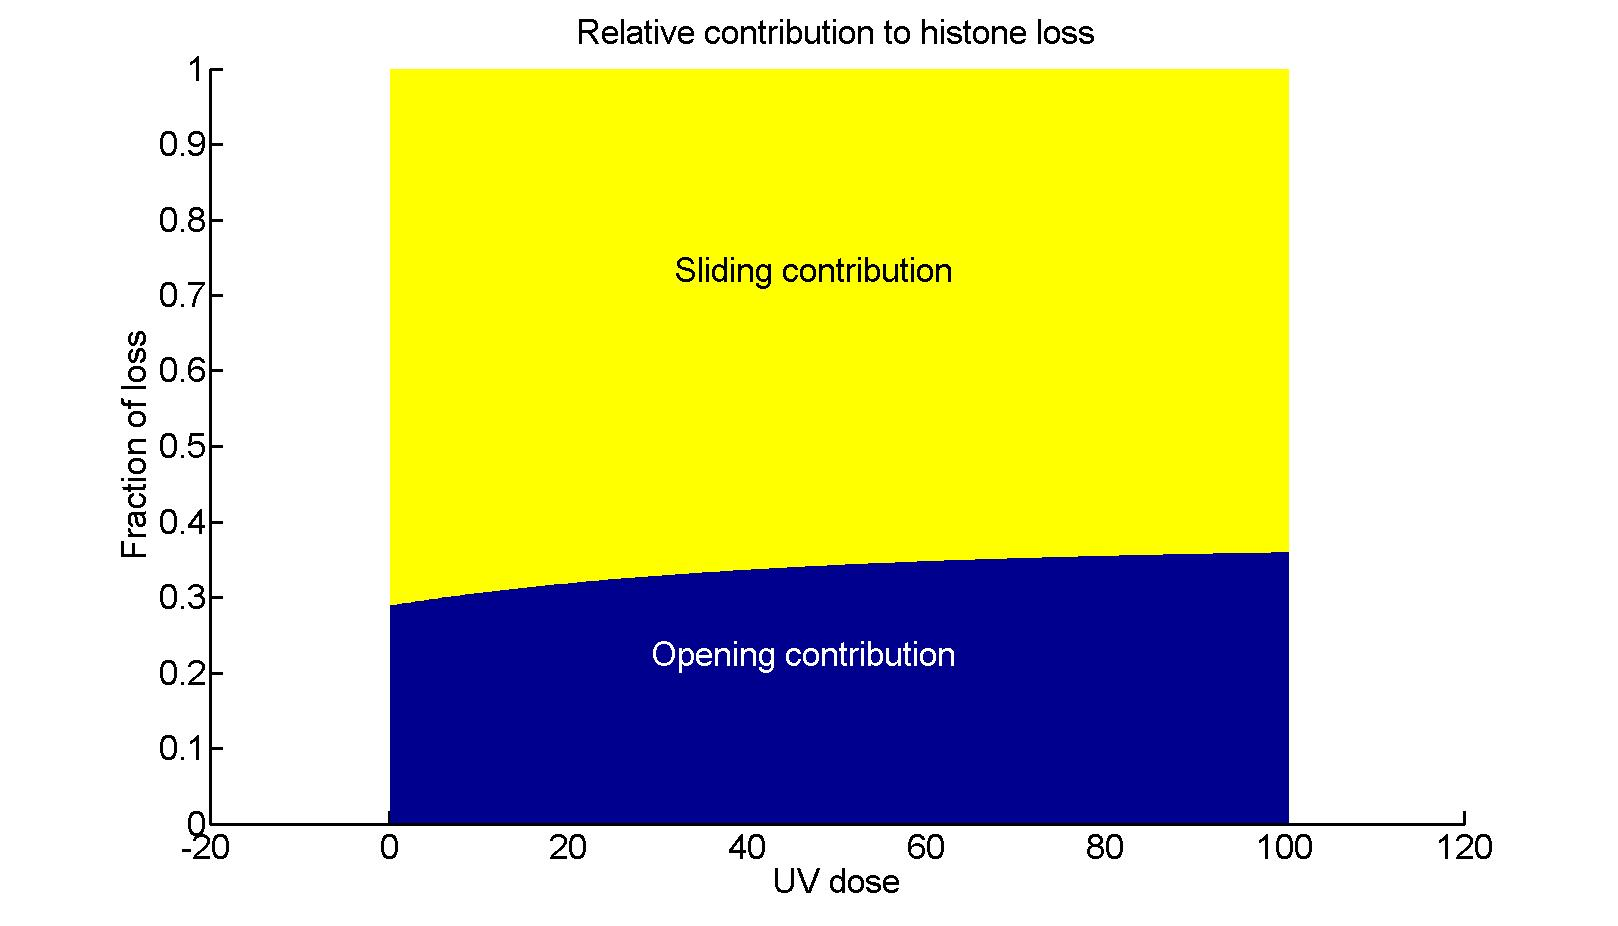
\includegraphics[width=0.5\linewidth, height=0.3\textheight]{relativeContributionToHistoneLoss}
	\caption{\textbf{Relative contribution of chromatin opening and histone sliding to DNA (left) and histone (right) loss}. Sliding contribution is monotonically decreasing with UV dose for both DNA and nucleosome signals. The increase in chromatin opening contribution is due to the increase in chromatin reorganization following high dosages of UV, which is responsible for the majority of signal loss}
	\label{fig:relatiiveContributionToLoss}
\end{figure}

\section{Material and methods: Modeling  histones and DNA redistribution following UV damages}
We present here a model for nucleosomes and DNA re-organization following UV damages. The cascade of events leading to tagged DNA and nuclesoms'  redistribution, results in signal extrusion from a region of interest (ROI) up to a maximal loss, measured 15 minutes post UVC. 

\subsection{Dynamics of histones following UV damages in the region of interest}

Following the experimental protocol, a 2D circular initial damage region (IDR), induced by the UV laser beam, is centered around the focal point (origin of the coordinates) with a fixed area of $A_0$. Following laser induction with UV dose, $u$, the tagged damage region expands radially outward and reaches it maximal area of $A(u)$ after 15 minutes. At the end of expansion, the circular region, characterized by $A(u)$, is defined as the ROI, which remains a fixed region for the measurement of signals at time 0 and 15 minutes. The fraction of signal loss is obtained by the ratio between measurements at the two times (see also the empirical definition in XXX). 

We assume that the loss of DNA and nucleosomes signal post UVC is due to two mechanisms: the first is chromatin expansion, and the second is nucleosomes sliding along the chromatin. In the first mechanism, recruitment and binding of repair factors to damaged DNA causes chromatin de-compaction, release of cross-links, and expansion of the chromatin in the IDR. Because the majority of damages are inflicted around the laser's focal point, the accumulation of repair factors will cause pushing force to surrounding chromatin in a radial outward direction, which result in DNA and nucleosome extrusion from the ROI in equal proportions. In the second mechanism, repair factors slide nucleosomes along the chromatin to facilitate efficient repair of DNA by exposing the damaged positions. 
Sliding nucleosomes over damaged positions on the DNA displaces the tagged damages spatially in the general direction of the ROI, and expand the IDR. 
 
Using the description above, we construct a model representing signal loss 15 minutes post UVC. We do not specifically take into account the mechanism of signal loss in time and only model the steady-state equations as a function of the UV dose.

\subsection{Fraction of DNA and nucleosome loss }\label{subsection:fractionOfDNAandNucleosomeLoss}
We assume an initial uniform distribution of both DNA and nucleosome. 
In our model, we set the number of nucleosomes in the IDR as $N(u)$. The ROI is considered to be a 2-dimensional circular region with an area $A(u)$, and the circular IDR of area $A_0$. 
We shall now compute the fraction of DNA loss (resp. nucleosomes) $D(u)$ (resp. $H(u)$) in the ROI 15 minutes post UVC. 

By construction, DNA signal loss is given by the ratio of the amount of DNA in the annulus between the IDR and the ROI to the total amount of signal in the ROI. Nucleosome signal loss is calculated as the sum of the nucleosomes that have been translocated with the DNA plus the ones that are sliding out, resulting in the following formulas
\begin{equation}\label{eq:DNAStSt}
D(u)= \frac{(A(u)/A_0) -1}{(A(u)/A_0)}
\end{equation}
\begin{equation}
\label{eq:histoneStSt}
H(u)=D(u)+\frac{N(0)-N(u)}{N(0)(A(u)/A_0)}.
\end{equation}
In order to evaluate the functions above, we will now construct models for the functions $A(u)$ and $N(u)$.

The increase of DNA damages with UV dose is thought of as governing the dynamics of both nucleosome and DNA signal loss. Therefore, we start our construction with a description of the accumulation of damages $T(u)$ in the IDR, and derive the function $N(u)$ and $A(u)$ from it.

\subsection{Deriving the number of damages $T(u)$}
We assume here that the rate of accumulating DNA damages, $T(u)$, with increasing uv dose in the IDR is increasing proportional to the undamaged DNA in the IDR.
\begin{equation}
\frac{dT(u)}{du}=k_T\left(T_{max}-T(u)\right)
\end{equation}
with $k_T$ the rate constant, and $T_{max}$ the maximal number of damages possible in $A_0$. 
Using the initial condition $T(0) = 0$ the solution is
\begin{equation}
T(u) = T_{max}\left(1-\exp(-k_T u)\right) 
\end{equation}
We assume no two damages can occur in the same position on the DNA, hence we can treat the quantity 
\begin{equation*}
T(u)/T_{max}
\end{equation*}
as the fraction of chromatin length in the IDR which is damaged, or as the DNA damage -coverage percentage. 

\subsection{Deriving the function $A(u)$ and $N(u)$}
We now turn to construct a model for the number of nucleosomes $N(u)$ left in ROI, as a function of the UV dose. Although the exact mechanism by which nucleosomes are lost is not known, we assume here that the number of nucleosomes leaving the ROI,namely  $N_0-N(u)$, is proportional to the rate of accumulation of DNA damages, $T(u)$, on nucleosomes. The nucleosmes occupy a length of the chromatin proportional to $N(u)$, whereas chromatin damage coverage is proportional to $T(u)$. Therefore, in the first-order approximation, the dynamics of $N(u)$ is given as by the multiplication 

\begin{equation*}
\frac{dN(u)}{du} = -k_N\frac{N(u)}{T_{max}}\frac{dT(u)}{du}
\end{equation*}
with $k_N$ a constant describing the rate of nucleosome depletion from the ROI due to sliding. Using the initial condition $N(0) = N_0$, the solution is given by
\begin{equation}\label{eq:NumHistones}
N(u) = N_0\exp\left(-k_N\frac{T(u)}{T_{max}})\right).
\end{equation}

Next, we model the dynamics of the ROI area $A(u)$ with increasing UV dose.  For this end, we consider the ROI expansion to be affected by two additive mechanisms: one is chromatin de-compaction, and the other is nucleosome sliding. 

\begin{equation}\label{dralpha}
\frac{dA(u)}{du}=-k_A\frac{dN(u)}{du}+k_B\frac{dT(u)}{du}
\end{equation}
where $k_A$ is a constant. Using the initial condition $A(0)=A_0$, we find 
\begin{equation}\label{eq:RoiArea}
A(u) = A_0 +k_AN_0\left(1-\frac{N(u)}{N_0})\right) +k_BT(u)
\end{equation}
where $A_0$ represents the size of the IDR even in the absence of UV induction.

We can now substitute equations \ref{eq:NumHistones} and \ref{eq:RoiArea} into the steady-state equation \ref{eq:DNAStSt} and \ref{eq:histoneStSt} to get the expressions 
\begin{equation}
\label{eq:DnaLoss}
D(u) = \frac{k_AN_0\left(1-\exp\left(-k_NT(u)/T_{max}\right)\right) +k_BT(u)}{A_0+k_AN_0\left(1-\exp\left(-k_NT(u)/T_{max}\right)\right) +k_BT(u)}
\end{equation}
and 
\begin{equation}\label{eq:histoneLoss}
H(u) = 1- \frac{\exp\left(-k_NT(u)/T_{max}\right)}{1+\frac{k_AN_0}{A_0}\left(1-\exp\left(-k_NT(u)/T_{max}\right)\right) +\frac{k_B}{A_0}T(u)}
\end{equation}


\subsection{Parameter fit for $H(u)$ and $D(u)$ }\label{subsection:parameterFit}
We now use equations. \ref{eq:histoneLoss} to fit the experimental data describing the fraction of nucleosome loss from the ROI 15 minutes post UVC. Because $D(u)$ and $H(u)$ share similar parameters, only the H3.3 data will be used to fit the function $H(u)$ and he resulting parameters will be used in the model for $D(u)$. 
Excluding the measurement at $u=100$ ms and using classical fitting procedure, we find a $R^2= 0.94$ using the following parameters
\begin{eqnarray*}
k_T &=&  0.021\\
k_N &=&  0.39\\
\frac{k_AN_0}{A_0}&=& 0.44\\
\frac{k_BT_{max}}{A_0}&=& 0.23
\end{eqnarray*}

Plugging these values into DNA loss equation \ref{eq:DnaLoss} and calculating the deviation, we find a value of $R^2=0.87$
\begin{figure}[H]
\centering
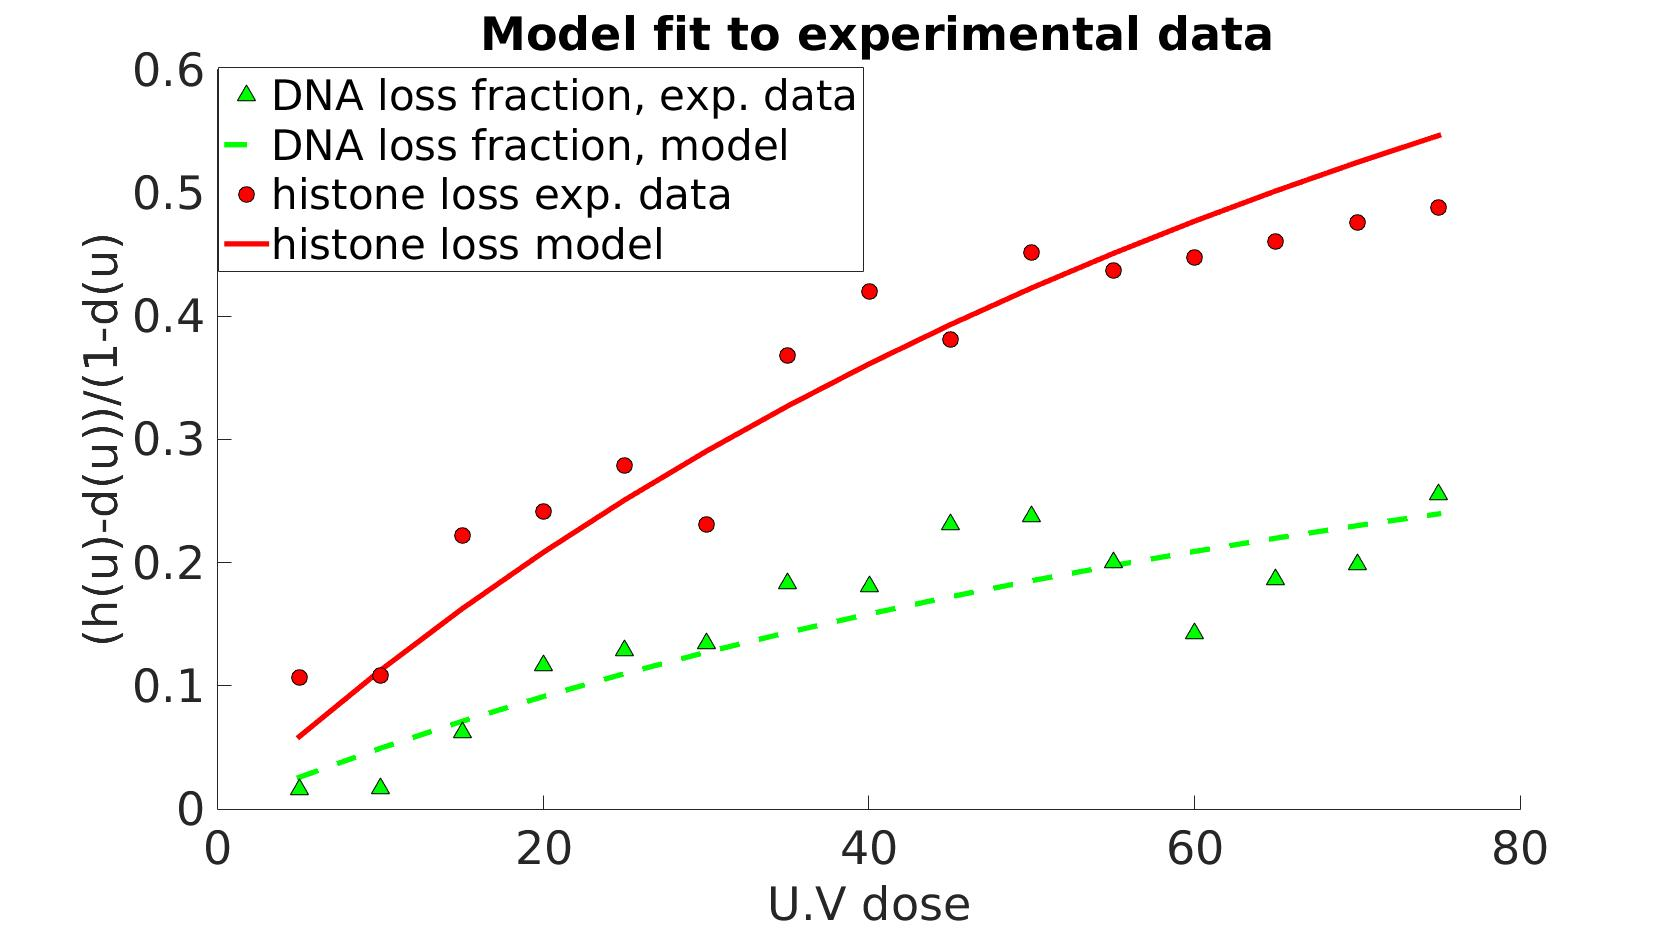
\includegraphics[width=0.6\linewidth, height=0.3\textheight]{histoneAndDnaVsUvDoseModelFit}
\caption{\textbf{Histone loss (red): experimental data (circle) versus analytical curve (continuous)}. The fit is obtained from  eq. \ref{eq:histoneLoss}. The parameters found in fitting of the H3.3 loss signal are plugged into equation \ref{eq:DnaLoss} for DNA signal loss (green dashed curve) and plotted against experimental points (green triangles).}
\label{fig:histoneAndDnaVsUvDoseModelFit}
\end{figure}

\subsection{Relative contribution of opening and sliding to DNA and nucleosome signal loss}
Using the calibrated model in equation \ref{eq:DnaLoss} and \ref{eq:histoneLoss}, we now calculate the relative contribution of chromatin opening and nucleosome sliding to the total loss of DNA and nucleosomes.
We start by partitioning the ROI area dynamics into the two sub-mechanisms of signal loss
\begin{equation*}
A(u) = A(u)_{opening}+A(u)_{sliding}
\end{equation*}

The effect of de-compaction on the expansion of the damage region and loss of signal is given by the second term on the right hand-side of equation \ref{dralpha}. Zeroing-out the sliding contribution term and,  we obtain an equation for the opening contribution 
\begin{equation*}
\frac{dA(u)_{opening}}{du}=k_B\frac{dT(u)}{du}
\end{equation*}
with the initial condition $A(0)_{opening}=A_0$, the solution is given by
\begin{equation}
A(u)_{opening}= A(0)+k_BT_{max}(1-\exp(-k_Tu))
\end{equation}
The fraction attributed to opening out of the total DNA loss due is given by 
\begin{equation}\label{eq:openingContributionDNA}
\frac{D(u)_{opening}}{D(u)}=\frac{\left(A(u)_{opening}/A_0\right)-1}{\left(A(u)/A_0\right) -1}
\end{equation}
and the complementary function 
\begin{equation}\label{eq:slidingContributionDNA}
\frac{D(u)_{sliding}}{D(u)}=1-\frac{D(u)_{opening}}{D(u)}
\end{equation}
indicates the relative contribution of sliding to the total DNA loss. 

Similarly, the relative contribution of opening to the total nucleosome loss is given by 
\begin{equation}\label{eq:openingContributionHistones}
\frac{H_{opening}}{H(u)} =\frac{\left(A(0)_{opening}/A_0\right)-1}{(A(u)/A_0)-(N(u)/N_0)}
\end{equation}
and for sliding
\begin{equation}\label{eq:slidingContributionHistones}
\frac{H_{sliding}}{H(u)} = 1-\frac{H(u)_{opening}}{H(u)} 
\end{equation}
where here we used the fact that $H(u)_{opening}=D(u)_{opening}$
The result can be appreciated in Figure \ref{fig:relatiiveContributionToLoss}, where the sliding contribution for both DNA and nucleosome loss is a decreasing function of the UV dose. 

\subsection{Nucleosomes sliding out of the IDR}
The fraction of nucleosomes sliding ot of the IDR (and eventually pushed out of the ROI) is given by the expression 
\begin{equation}
\frac{H(u)-D(u)}{1-D(u)}
\end{equation}
Using the parameter values in subsection \ref{subsection:parameterFit} and plugging \ref{eq:histoneLoss} and \ref{eq:DnaLoss} into the expression above, we obtain the results in Figure \ref{fig:fractionSlidingOutOfIDR}, where the model is plotted against the experimental data ($R^2=0.89$). 

\begin{figure}[H]
\centering
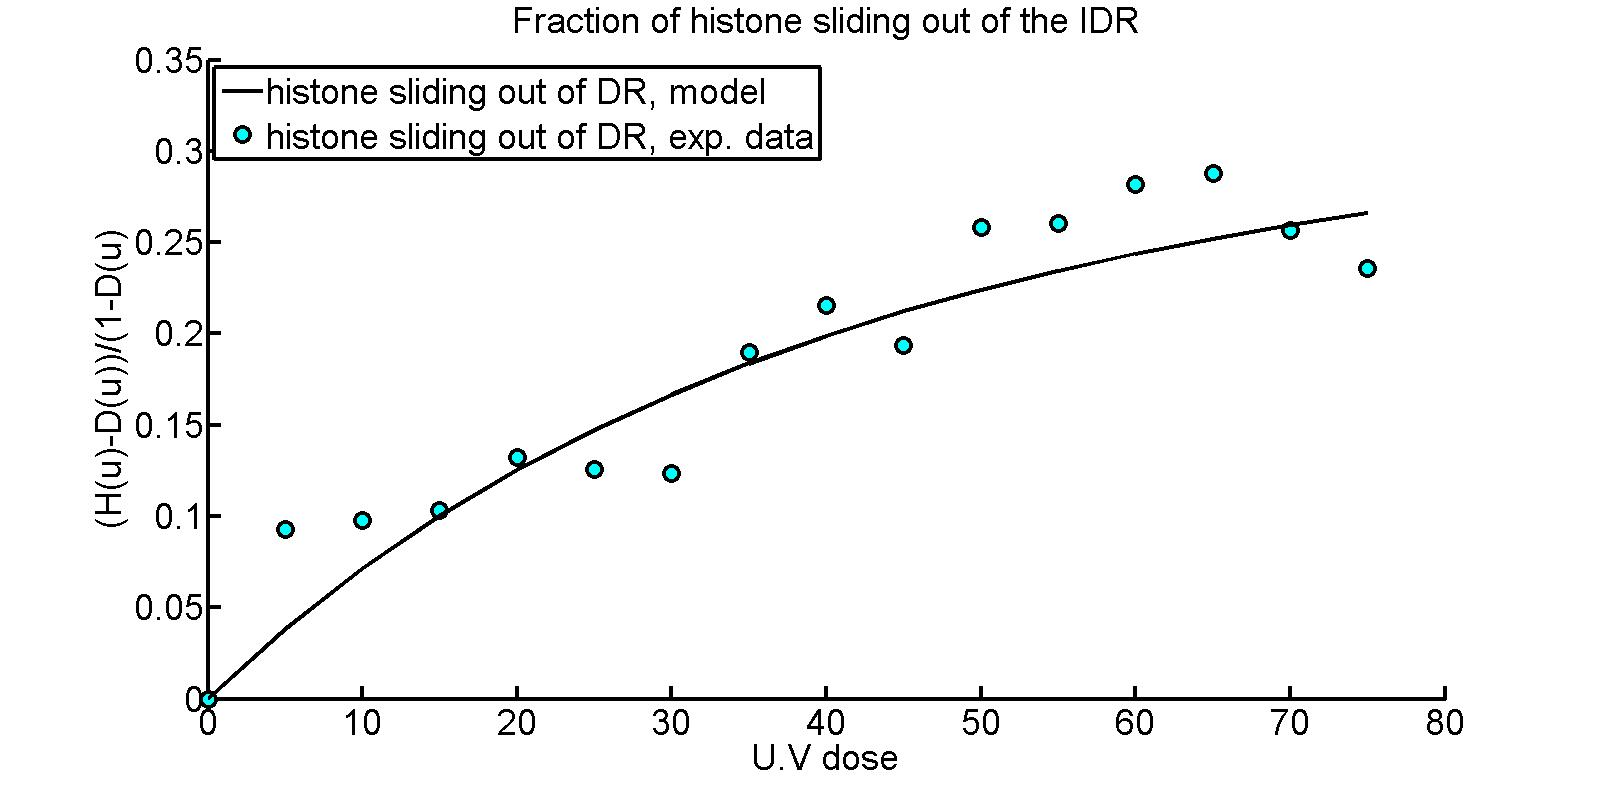
\includegraphics[width=0.5\linewidth, height=0.3\textheight]{fractionSlidingOutOfIDR}
\caption{\textbf{Fraction of nucleosomes sliding out of the IDR.The plot against the experimental data results in $R^2=0.89$ }}
\label{fig:fractionSlidingOutOfIDR}
\end{figure}


\end{document}

